
\section{\zkwasm\ Architecture Circuits}
\label{chp:architecture-circuits}

As we have prepared our circuit building blocks in Section \ref{chp:build-blocks}, we can start constructing the main circuits involved in \zkwasm. We will first describe the workflow of \zkwasm\, by splitting it into four stages to give a big picture of how different circuits (see Figure \ref{fig:arch-circuits}) interplay with each other and then we will present the details of each circuit.

\begin{figure}[!ht]
\centerline{
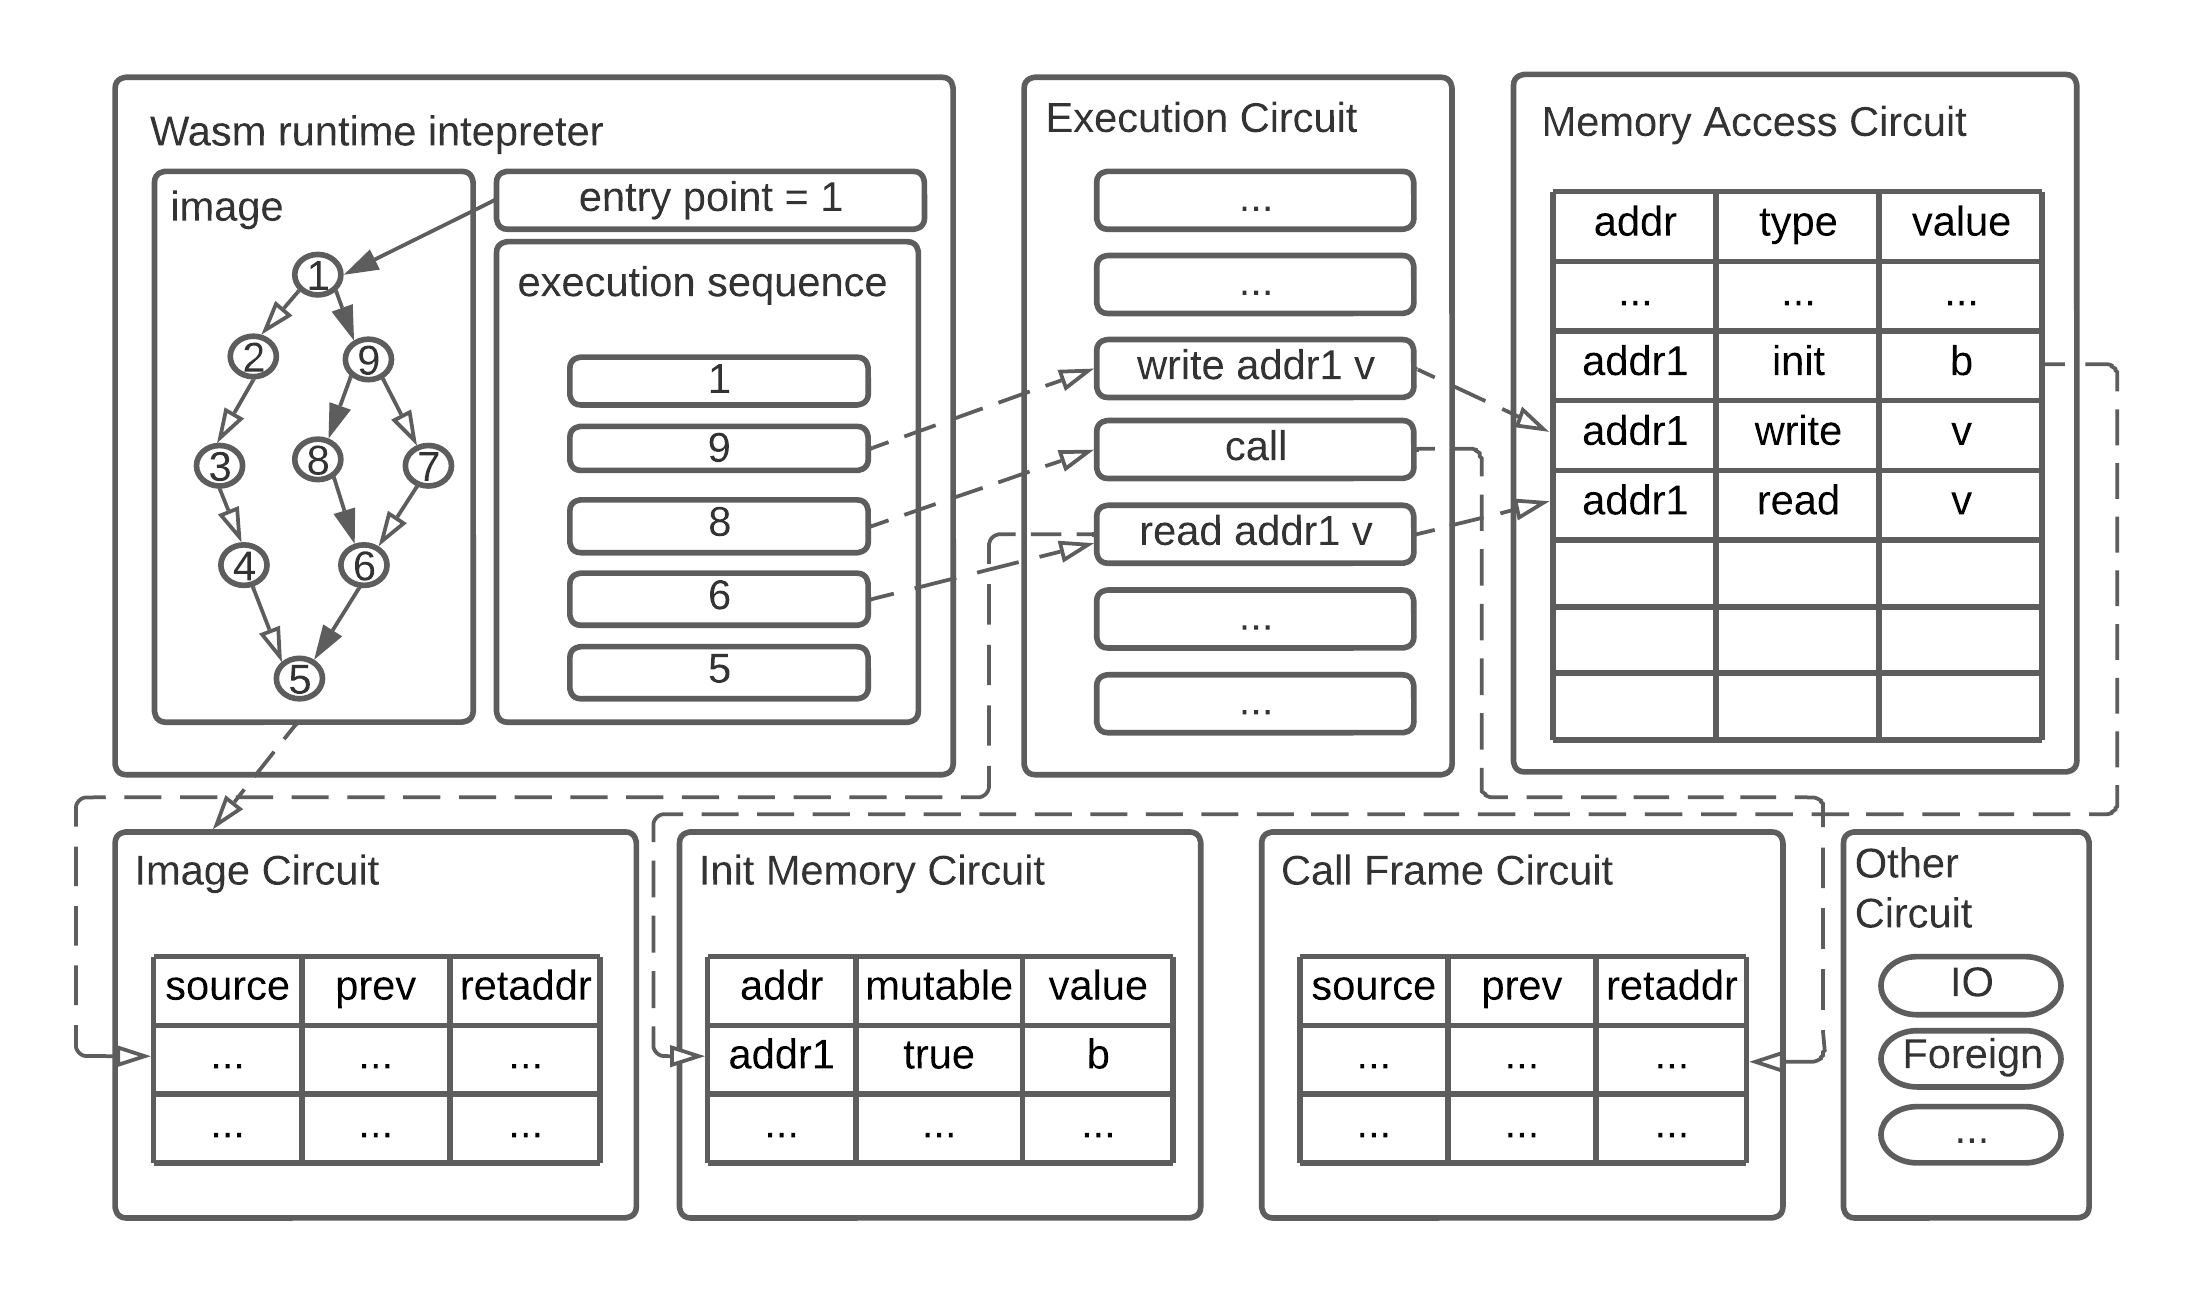
\includegraphics[scale=0.7]{figs/arch-circuits.png}
}
\caption{Architecture circuits}\label{fig:arch-circuits}
\end{figure}


\noindent\emph{Step 1: Image Setup.}
Defined by the WASM specification, a WASM image $\mathbf{I}$ is divided into sections. Among them, there are sections that do not affect the execution of WASM (custom section, type section, export section, data count section) and sections that decide the execution semantics (initial memory section, code section, global data section). At the image setup stage, we encode the code section into the lookup table $\mathbf{T}_\mathbf{I}$ and the data section into the lookup table $\mathbf{T}_\mathbf{H}$. These two tables will be used to enforce that each instruction in the execution trace is a valid instruction and that all the initialization of the memory access log table complies with the initial data section of image $I$.\\

\noindent\emph{Step 2: Execution Trace Generation.}
Recall that a valid execution trace is a sequence of transition functions $\left[t_0, t_1, \cdots\right]$ such that each $t_i$ is related to the 
$i$th instruction during the execution of $(\mathbf{I}, \mathbf{E}, \mathbf{IO})$. We uses the standard WASM run-time interpreter to generate ${t_i}$ that is valid as defined in Definition \ref{def:valid-trace}.
\begin{remark}
We do not require the WASM run-time interpreter to be a trust component since if it generates an invalid sequence, the constraints of the Execution Circuit fail because our Execution Circuit enforces the semantics of each instruction.
\end{remark}

\smallskip\noindent\emph{Step 3: Synthesis Circuits.}
Once a valid execution trace is generated, it can be used to fill our main execution circuit $\mathbf{T}_\mathcal{E}$, together with other lookup tables $\mathbf{T}_\mathcal{F}$ (calling frame table), $\mathbf{T}_\mathcal{M}$ (memory access log table), $\mathbf{T}_\mathcal{G}$ (global access log table) and $\mathbf{T}_{\mathcal{SP}}$ (stack access log table). \\

\noindent\emph{Step 4: Proof Generation.}
After all the circuits are synthesised, we can generate a ZKSNARK proof via Halo2's proof system. The proof can be used to prove that the execution trace and its output are valid.

\subsection{Setup Circuits}
Setup circuits are filled by the \zkwasm\, compiler component and its purpose is to provide lookup tables $\mathbf{T}_\mathcal{C}$, $\mathbf{T}_\mathcal{H}$, $\mathbf{T}_\mathcal{G}$ that encode code section, initial memory section and global data section.\\

\noindent\emph{Code Section.}
The elementary items in the code section are $opcode$s of instructions that are grouped in a tree-like hierarchy. Each instruction can be indexed by $moid$ (modular id), $mmid$ (memory block instance id), $fid$ (function id) and $iid$ (offset of the instruction in a particular function). We denote $iaddr$ to be the tuple of $(moid, mmid, fid, iid)$ and represent the code section as a map from $iaddr$ to $opcode$. Using the technique in Section \ref{chp:map-repr}, it is equivalent to encoding the code section into $\mathbf{T}_\mathcal{C}$ (see Table \ref{tbl:code-table}). Code table $\mathbf{T}_\mathcal{C}$ is later used to constrain entries in execution table $\mathbf{T}_\mathcal{E}$ (see Section \ref{chp:ex-table}) such that if $e \in \mathbf{T}_\mathcal{E}$ then $(e.iaddr, e.opcode)$ must also in $\mathbf{T}_\mathcal{C}$. 

\begin{table}[!h]
\begin{center}
\caption{Code table}
\label{tbl:code-table}
\begin{tabular}{ | c | c | c | c | c | }
  \hline
  moid & mmid & fid & iid & opcode \\
  \hline
  $0x00$ & $0x01$ & $0x01$ & $0x00$ & $add$ \\
  \hline
  $0x00$ & $0x01$ & $0x01$ & $0x01$ & $sub$ \\ 
  \hline
  $\cdots$ & $\cdots$ & $\cdots$ & $\cdots$ & sub \\ 
  \hline
\end{tabular}

\end{center}
\end{table}

\noindent\emph{Initial Memory \& Global Data.}
The element items in the memory section of WASM image are unsigned 64 bit words (u64). The address of each $u64$ word can be indexed by $mmid$ and $offset$. Besides the value, memory can have types that are either mutable or immutable. Thus the memory section can be represented as a map from $(mmid, offset)$ to $(value, isMutable)$. Similarly, using the technique in Section \ref{chp:map-repr}, we can encode the initial memory section into $\mathbf{T}_\mathcal{H}$. Similar to the init memory section, the global data section contains variable instances that can be shared between different modules which can also be represented as a map from $(mmid, offset)$ to $(value, isMutable)$. Thus we merge two tables into one and use $ltype = Memory \,|\, Global$ to distinguish them (see Table \ref{tbl:init-memory-table} for an example of $\mathbf{T}_{\mathcal{H}}$).
\begin{table}[!h]
\begin{center}
\caption{Initial memory table}
\label{tbl:init-memory-table}
\begin{tabular}{ | c | c | c | c | c | }
  \hline
  $ltype$ & $mmid$ & \emph{offset} & $value$ & $isMutable$ \\
  \hline
  $Heap$ & $mmid_0$ & $1$ & $0x01$ & $true$ \\
  \hline
  $Heap$ & $mmid_1$ & $1$ & $0x01$ & $true$ \\
  \hline
  $Global$ & $mmid_2$ & $1$ & $0x01$ & $true$ \\ 
  \hline
  $Global$ & $mmid_3$ & $1$ & $0x01$ & $false$ \\ 
  \hline
\end{tabular}

\end{center}
\end{table}

We use $\mathbf{T}_\mathcal{H}$ to constrains entries in the memory access log table $\mathbf{T}_\mathcal{M}$ (see Table \ref{tbl:rw-table}) so that $\forall e, e\in \mathbf{T}_\mathcal{M} \wedge e.accessType = Init \rightarrow (e.iaddr, value) \in \mathbf{T}_\mathcal{H}$. The meaning of this constraint is that for each init access log in $\mathbf{T}_\mathcal{M}$ it must be defined in the initial memory section or global data section.


\subsection{Execution Trace Circuits}
\label{chp:ex-table}
Execution Trace Circuits are used to constraint the execution trace $\left[t_0,t_1,t_2,\cdots\right]$ (see Section \ref{chp:exec-trace}) emulated from WASMI (WASM interpreter). Each trace element is related to an instruction in the code table $\mathbf{T}_\mathcal{C}$ and has a predefined semantic based on the opcode. The semantics of a WASM opcode is defined based on its parameters derived from the stack and the micro operations. First, since WASM is a stack machine, we define the \emph{operands} of an opcode $op$ to be
\[
operands(op) = p_0, p_1, p_2 \cdots, p_k
\]
where $p_i$ are values on the stack and $p_i = stack[sp+i]$.
Second, we define the semantics of $op$ by a sequence of microoperations
\[
mop_i = \begin{cases}
    w_i = load(ltype, addr)\, \textnormal{ where $addr \in \{p_1, p_2, \cdots, p_k, w_0, w_1, \cdots, w_{i-1}\}$}\\
    write(ltype, addr, v)\, \textnormal{ where $addr, v \in \{p_1, p_2, \cdots, p_k, w_0, w_1, \cdots, w_{i-1}\}$}\\
    w_i = arith(p_1, p_2,\cdots, p_k, w_0, w_1, \cdots, w_{i-1}); \\
    \textit{FALLTHOUGH}; \\
    GOTO(iaddr); \\
    if \, b\, then\, \{mop_{i+1}, \cdots mop_{j}\} \,else\, \{mop_{j+1},\cdots\}.
    \end{cases}
\]
When filling execution trace into the execution circuit, we arrange the instruction into small blocks (see Table \ref{tbl:ex-table}) of the execution circuit such that each block represents an instruction. Within each block, we use the $start$ column to indicate whether this row is the start of a new instruction block and put $op$ and $mop$ in the opcode column. In the address column, we push all used addresses and the first row is the instruction address of this instruction in $\mathbf{T}_\mathcal{C}$ and in the $sp$ column we record all the changes of stack pointer.
\begin{table}[!h]
\begin{center}
\caption{Execution table}
\label{tbl:ex-table}
\begin{tabular}{ | c | c | c | c | c | c | c | c | c | c | }
  \hline
  start & opcode & bit cell & state & aux & $address \in T_{I}$ & $sp$ & u64 cell \\ 
  \hline
   true & $op$ & $b_0$ & $tid_0$ & $aux$ & $iaddr_0$ & $sp$ & $w_0$ \\ 
 \hline
   0 & $mop_0$ & $b_1$ & $frame$ & $aux_0$ & $addr_0$ & $\cdots$ & $w_1$ \\ 
 \hline
   0 & $mop_1$ & $b_2$ & $..$ & $aux_1$ & $addr_1$ & $\cdots$ & $w_2$ \\ 
 \hline 
  0 & $mop_2$ & $b_3$ & $s_3$ & $aux_2$ & $addr_2$ & $\cdots$ & $w_3$ \\ 
 \hline
   $\cdots$ & $\cdots$ & $\cdots$ & $\cdots$ & $\cdots$ & $\cdots$ & $\cdots$ & $\cdots$ \\ 
 \hline
   true & $op_1$ & $b$ & $tid_1$ & $aux$ & $iaddr_1$ & sp' & $w$ \\ 
 \hline
   $\cdots$ & $\cdots$ & $\cdots$ & $\cdots$ & $\cdots$ & $\cdots$ & $\cdots$ & $\cdots$ \\
 \hline
 \hline
\end{tabular}

\end{center}
\end{table}

\smallskip Although different opcodes might have different semantics thus different $mop_k$, $addr_i$, etc. There are some common constraints that we need to enforce in the execution circuit. First. we need to enforce that each instruction exists in the code section, thus $(iaddr, opcode) \in \mathbf{T}_\mathcal{C}$. Second, suppose that $operand$ $p_i$ is got from stack pointer $sp$ as a result of $mop_k(sp)$, then $(sp, read, iaddr, k, p_i) \in \mathbf{T}_{\mathcal{M}}$, which means the result $p_i$ is enforced from a valid memory access log table. Similarly, suppose that witness $w_i$ is got from memory access of $addr_j$ with access type $ltype$ as a result of $mop_k$, then $(mem, addr_j, ltype, k, w_i) \in \mathbf{T}_{\mathcal{M}}$.  Third, we enforce that all the cells in bit column are either zero or one and all the cells in u64 witness column and operand column are in $\mathbf{T}_{64}$ (less than $2^{64}$).

\subsection{Frame Circuit}
\label{chp:frame-circuit}
Frame Circuit is a table (see Figure \ref{fig:frame-circuit}) that helps us to find out the next $iaddr$ of the return instruction (see Section \ref{chp:control-flow-ins}). Each entry of $\mathbf{T}_\mathcal{F}$ is a tuple of $(prevFrame, currentFrame, iaddr)$  where $currentFrame$ is the tid of the call instruction that starts this call frame, $prevFrame$ is the $tid$ of the call instruction of previous call frame and $iaddr$ is the call instruction address of the current call frame. Suppose that $t_i$ is a return instruction at state $s_i$ with $(currentFrame, prevFrame)$ and the state $s_{i+1} = t_i \circ t_{i-1} \circ \cdots t_0(s_0)$, then we constrain that
\[
    plookup(\mathbf{T}_\mathcal{F}, (prevFrame, currentFrame, s_{i+1}.(iaddr-1))) = 0
\] to make sure the return address is correct (see Figure \ref{fig:frame-circuit}).
\begin{figure}[!h]
\centerline{
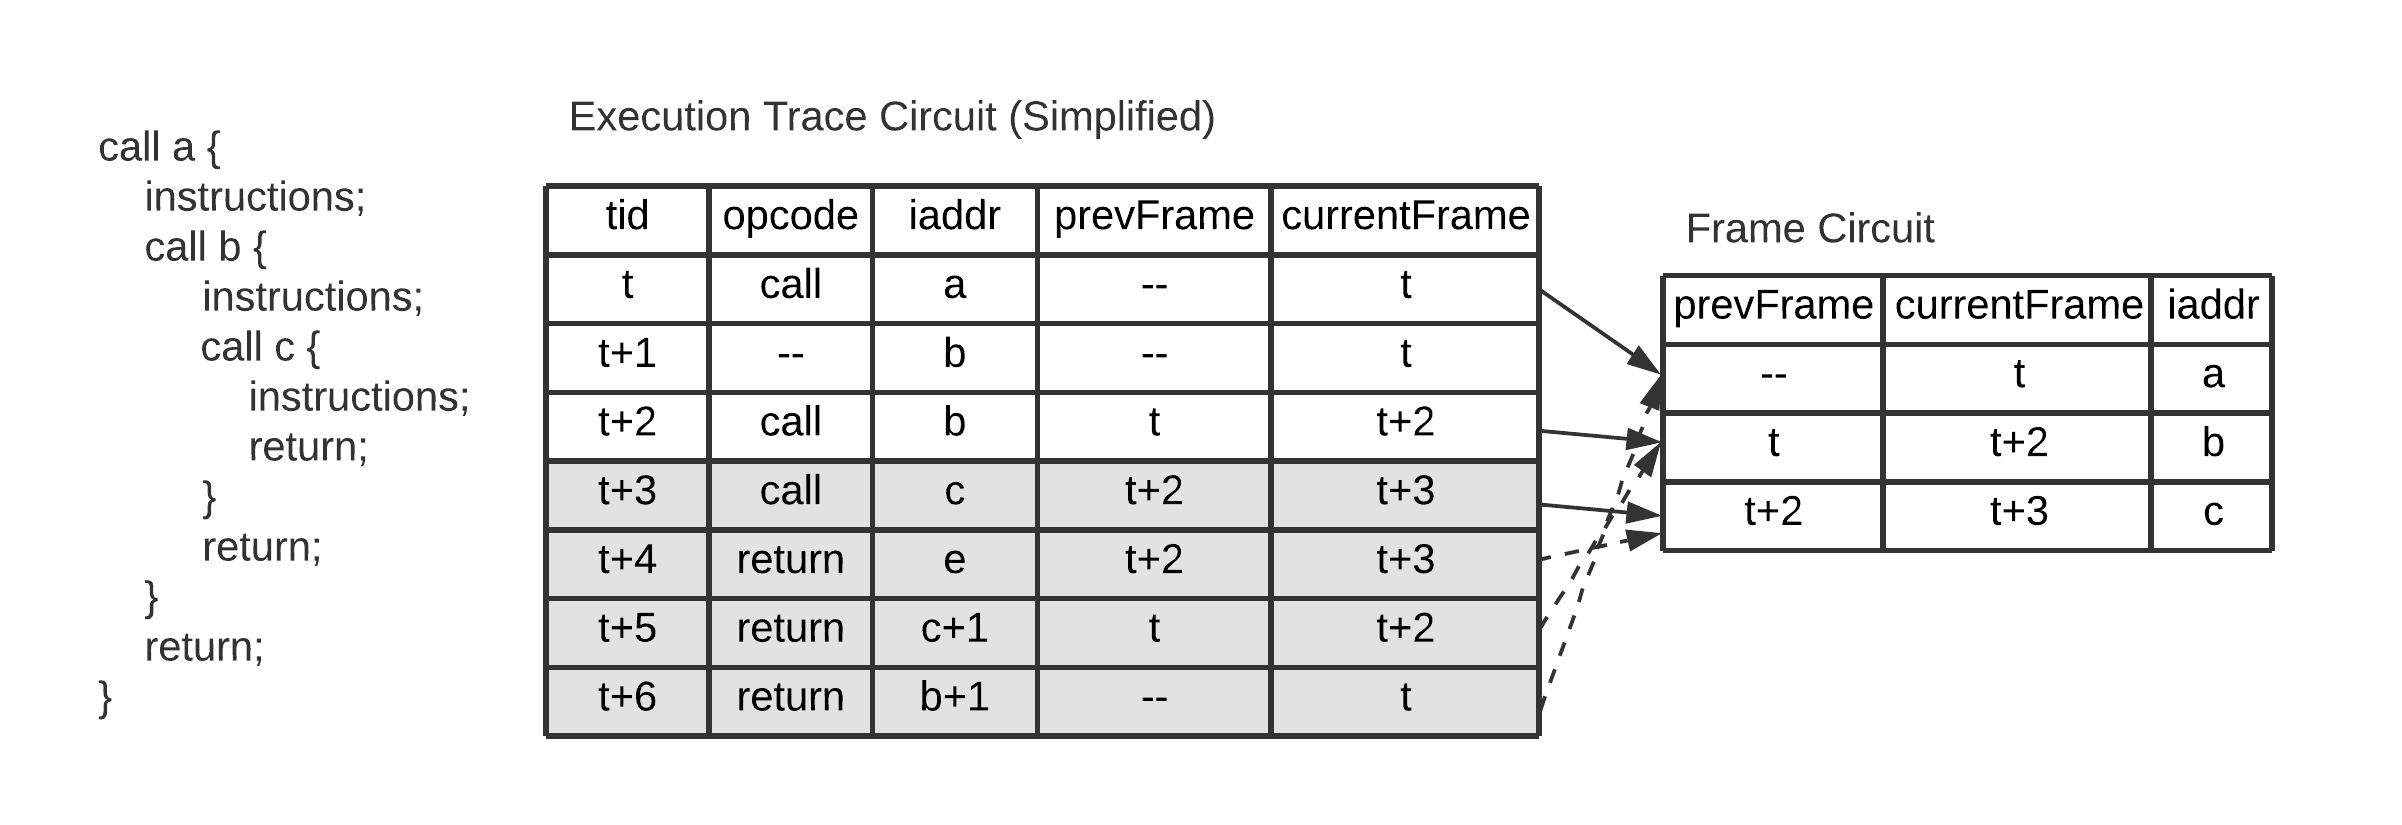
\includegraphics[scale=0.7]{figs/frame-circuit.png}
}
\caption{Frame circuit}\label{fig:frame-circuit}
\end{figure}

\subsection{Access Log Circuit}
\label{chp:access-log-circuit}
Recall that the access log circuit is a unique table corresponding to a valid memory access log sequence and satisfies Equation \ref{eq:rw-constraints}. In WASM specification, an access log is used for three different types that are memory access, stack access and global access. Each access log has a type field that is either \emph{Init}, \emph{Read} or \emph{Write} and all logs are sorted by $(address, (tid, tmid))$ where $address$ is indexed by $ (mmid, offset)$, $tid$ is the transition index of the execution log that contains the access and $tmid$ is the index of the access micro-op in that instruction (see Table \ref{tbl:rw-table}).

\subsection{IO Circuits that Support Zero-knowledge}
Zero-knowledge of inputs is not supported in WASM specification. Thus to support the private inputs which we do not want to leak, we need to add special instructions in the \zkwasm\, to distinguish between private and public inputs. We represent public inputs in a separate column and use the polynomial lookup to link input values with the result of \emph{get\_public\_input(inputCursor)} (See Figure \ref{fig:public-input}).
\begin{figure}[!ht]
\centerline{
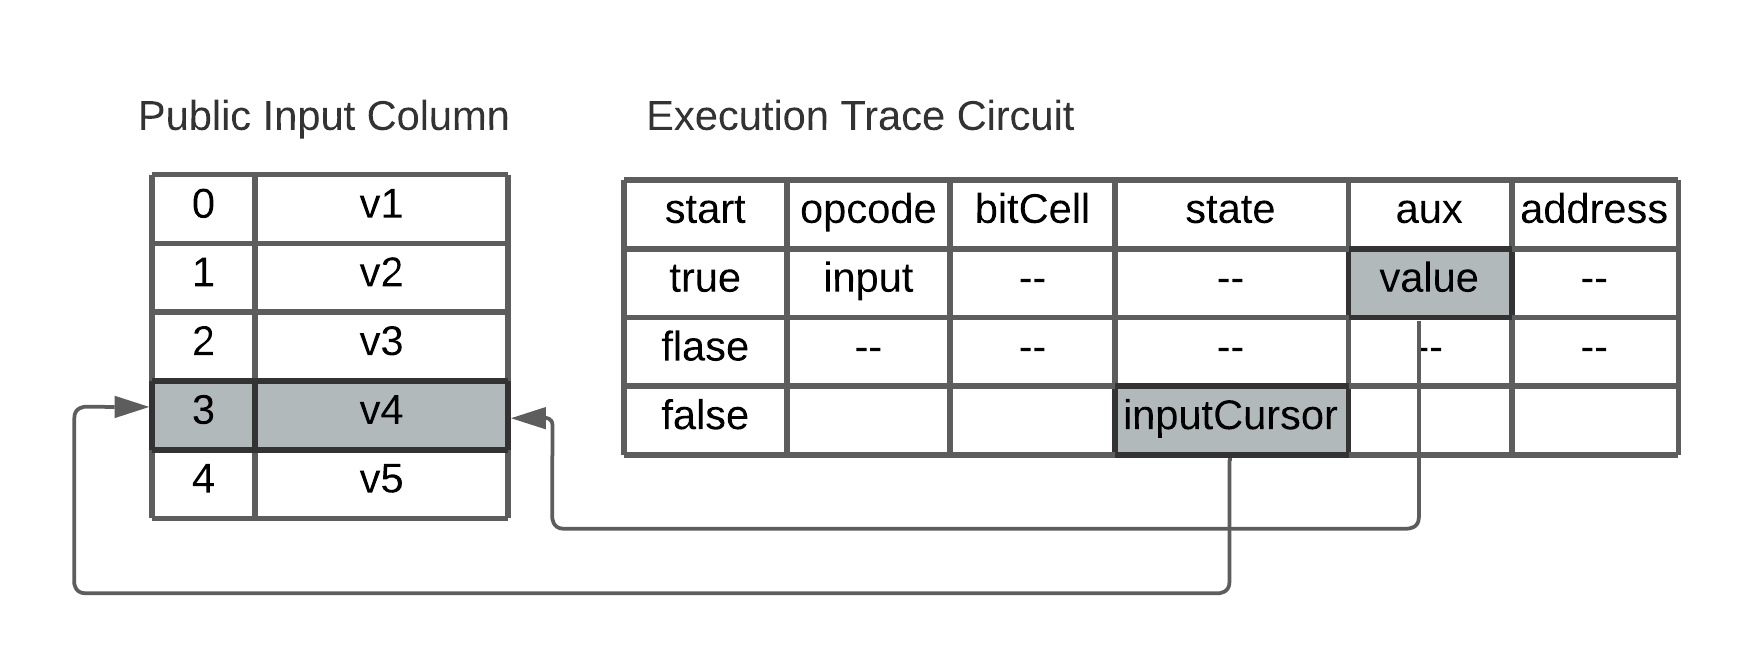
\includegraphics[scale=0.7]{figs/public-input.png}
}
\caption{Public input circuit}\label{fig:public-input}
\end{figure}
 Similarly, we use a separate column to hold output data and use a polynomial lookup to enforce that the value we output in the execution circuit $aux$ cell lies in the output column. When dealing with private inputs from $\emph{get\_private\_input(inputCursor)}$, we put them into the related cell with no constraints as the proof system will hide the value for us.